\documentclass[xcolor={rgb}]{beamer}
\usefonttheme[onlymath]{serif}
\usepackage[labelformat=empty]{caption}
\usepackage[outputdir=out]{minted}

\usetheme{Cuerna}

\author{Alireza Arzehgar}
\title{Implement Fourier Serie Using C}
\institute{Azad University of Mashhad}
\date{\today}

\begin{document}
	\begin{frame}[plain]
		\titlepage
	\end{frame}

	\begin{frame}{What is Fourier Serie?}
		\pause
		\[ f(x) = a_0 + \sum_{n=1}^{\infty}a_n \cos(\frac{n \pi x}{L})+b_n \sin(\frac{n \pi x}{L}) \]
		\pause
		\[ a_0 = \frac1T \int_{-L}^{L} f(x)\mathrm{d}x \]
		\pause
		\[ a_n = \frac1L \int_{-L}^{L} f(x)\cos(\frac{n \pi x}{L})\mathrm{d}x \]
		\pause
		\[ b_n = \frac1L \int_{-L}^{L} f(x)\sin(\frac{n \pi x}{L})\mathrm{d}x \]
	\end{frame}
	
	\begin{frame}[fragile,c]{How to implement Integral programmatically?}
		\vspace*{0.5cm}
		\hspace*{0.5cm}
		\begin{overprint}
			\onslide<2>
			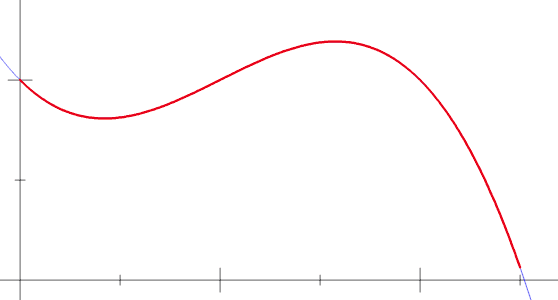
\includegraphics[width=\textwidth]{assets/int-0.png}
			\onslide<3>
			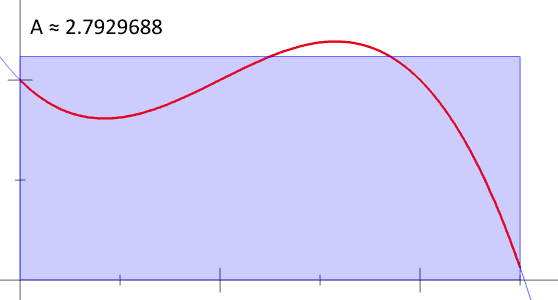
\includegraphics[width=\textwidth]{assets/int-1.png}
			\onslide<4>
			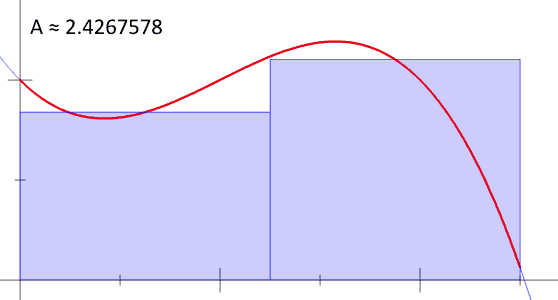
\includegraphics[width=\textwidth]{assets/int-2.png}
			\onslide<5>
			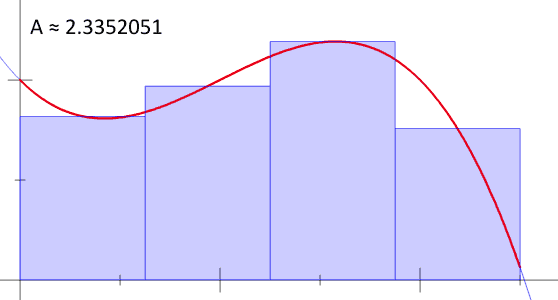
\includegraphics[width=\textwidth]{assets/int-3.png}
			\onslide<6>
			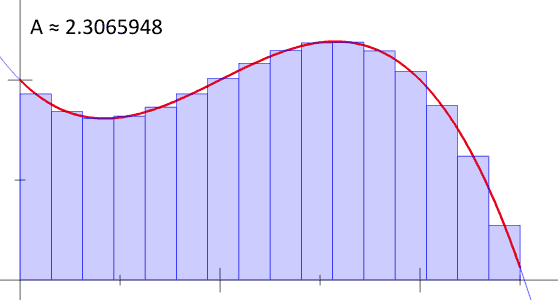
\includegraphics[width=\textwidth]{assets/int-4.png}

			\onslide<7>
			\vspace*{1cm}
			\begin{minted}{c}
double lowerl = -2, upperl = 4,
       p = 0.0001,  sum = 0;
for (double x = lowerl; x <= upperl; x += p)
	sum += x * p;

cout << sum << endl; // 5.9997
cout << round(sum * 100) / 100 << endl; // 6
			\end{minted}
		\end{overprint}
	\end{frame}

	\begin{frame}[fragile,c]{How to find fourier coefficients?}
		\footnotesize
		\begin{overprint}
			\onslide<2>
			\begin{minted}{c}
double lowerl = -M_PI, upperl = M_PI,
       L = (upperl - lowerl) / 2, p = 0.001;

for (int n = 0; n <= 5; n++) {
	double An = 0, Bn = 0;

	for (double x = lowerl; x <= upperl; x += p)
		An += (f(x) * cos(n * M_PI * x / L)) * p;
	An *= 1/L;

	for (double x = lowerl; x <= upperl; x += p)
		Bn += (f(x) * sin(n * M_PI * x / L)) * p;
	Bn *= 1/L;

	An = (abs(An) < 0.00001 ? 0 : An);
	Bn = (abs(Bn) < 0.00001 ? 0 : Bn);

	printf("A%d = %f, B%d = %f\n", n, An, n, Bn);
}
			\end{minted}

			\onslide<3>
			\[ a_n = \frac1L \int_{-L}^{L} f(x)\cos(\frac{n \pi x}{L})\mathrm{d}x \]

			\begin{minted}{c}
for (double x = lowerl; x <= upperl; x += p)
	An += (f(x) * cos(n * M_PI * x / L)) * p;
An *= 1/L;
			\end{minted}

			\[ b_n = \frac1L \int_{-L}^{L} f(x)\sin(\frac{n \pi x}{L})\mathrm{d}x \]

			\begin{minted}{c}
for (double x = lowerl; x <= upperl; x += p)
	Bn += (f(x) * sin(n * M_PI * x / L)) * p;
Bn *= 1/L;
			\end{minted}


			\onslide<4>
			\vspace*{1cm}
			For $f(x) = sin(x)$ in $-\pi < x < \pi$:

			\begin{minted}{text}
A0 = 0.000000, B0 = 0.000000
A1 = 0.000000, B1 = 1.000000
A2 = 0.000000, B2 = 0.000000
A3 = 0.000000, B3 = 0.000000
A4 = 0.000000, B4 = 0.000000
A5 = 0.000000, B5 = 0.000000
			\end{minted}

			\onslide<5>
			\vspace*{1cm}
			For $f(x) = x$ in $-2 < x < 2$:

			\begin{minted}{text}
A0 = 0.000000, B0 = 0.000000
A1 = 0.000000, B1 = 1.273239
A2 = 0.000000, B2 = -0.636619
A3 = 0.000000, B3 = 0.424412
A4 = 0.000000, B4 = -0.318309
A5 = 0.000000, B5 = 0.254647
			\end{minted}

			\onslide<6>
			\vspace*{1cm}
			For $f(x) = x^2$ in $-2 < x < 2$:

			\begin{minted}{text}
A0 = 2.668667, B0 = 0.000000
A1 = -1.623139, B1 = 0.000000
A2 = 0.407285, B2 = 0.000000
A3 = -0.182127, B3 = 0.000000
A4 = 0.103322, B4 = 0.000000
A5 = -0.066846, B5 = 0.000000
 			\end{minted}
			\end{overprint}
	\end{frame}


	\begin{frame}[fragile]{How to plot?}
		\onslide<+->
		\[ f(x) = \sum_{n=0}^{\infty}a_n \cos(\frac{n \pi x}{L})+b_n \sin(\frac{n \pi x}{L}) \]

		\begin{itemize}
			\pause\item Desmos
			\pause\item Gnuplot
			\pause\item Wolfram Mathematica
			\pause\item Programming Languages
		\end{itemize}
	\end{frame}

	\begin{frame}[fragile]{Plot our serie}
		\vspace*{1cm}
		\begin{overprint}
			\onslide<1>
			Generate part of fourier serie(for desmos calculator):
			\begin{minted}{c}
for (int n = 0; n <= 2; n++) {
	/* FIND COEFFICIENTS */
	printf("+%.2f\\cos(x*%d)", An, n);
	printf("+%.2f\\sin(x*%d)", Bn, n);
}
printf("\n");
// +-0.00\cos(x*0)+0.00\sin(x*0)+0.00\cos(x*1)
// +2.00\sin(x*1)+-0.00\cos(x*2)+-1.00\sin(x*2)
			\end{minted}
			\onslide<2>
			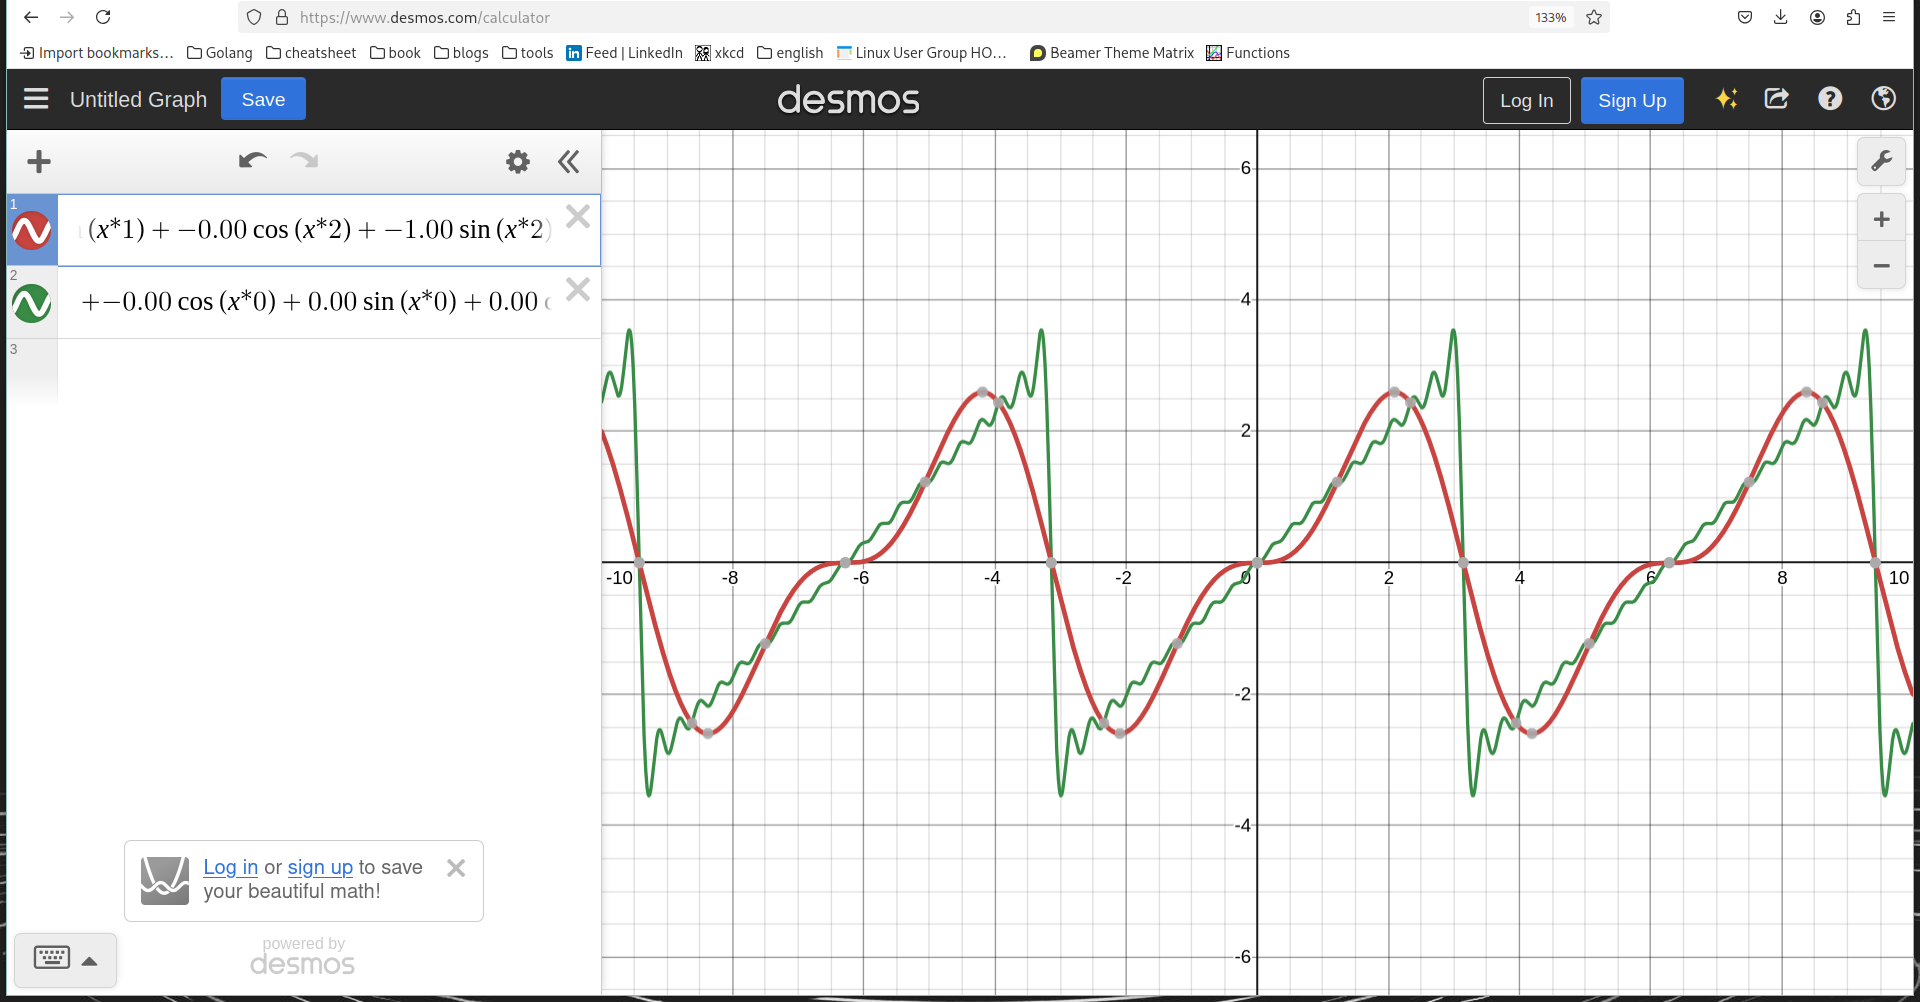
\includegraphics[width=\textwidth]{assets/desmos.png}
			\onslide<3>
			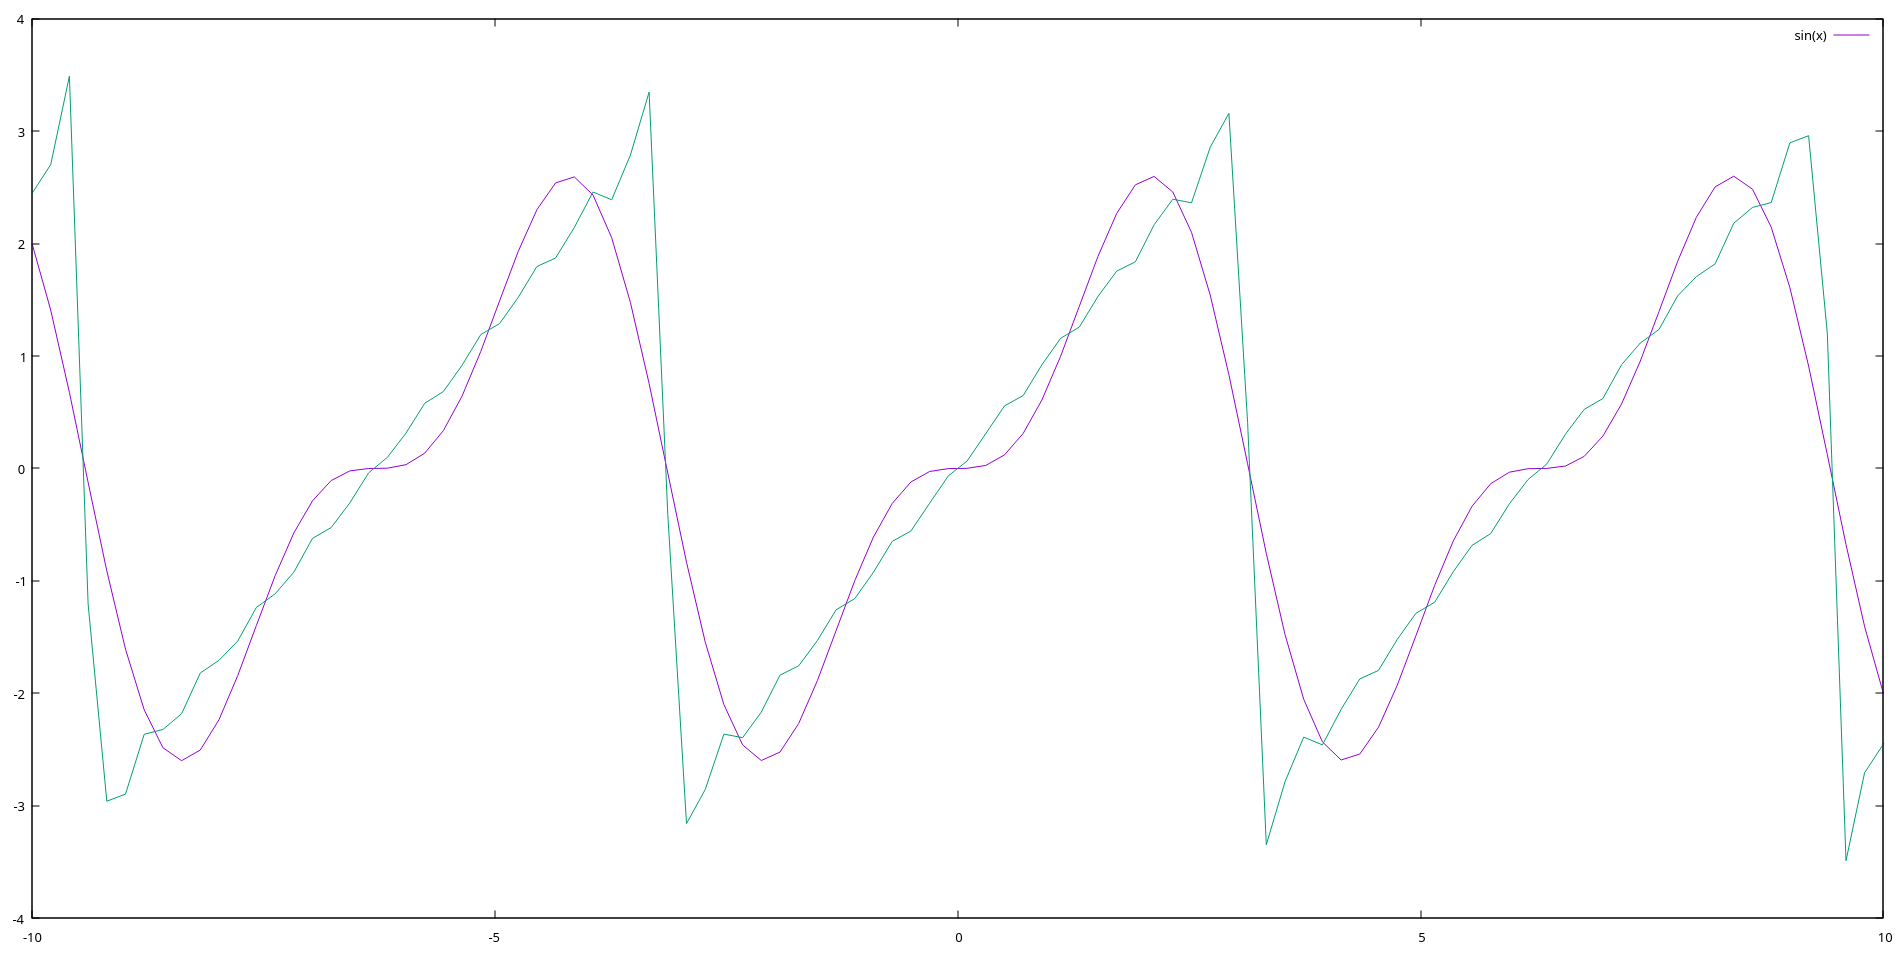
\includegraphics[width=\textwidth]{assets/gnuplot.png}
		\end{overprint}
	\end{frame}
\end{document}
